\section*{Cycle 1 Experiment 6}

\section{\Large{}}

\subsection{Aim}
\large To implement the Second Readers-Writers Problem.

\subsection{Theory}
The Readers-Writers problem is a classic synchronization problem.
\\
\\
\textbf{The problem statement }: There is a shared resource which should be accessed by multiple processes. There are two types of processes in this context: the reader and the writer. Any number of readers can read from the shared resource simultaneously, but only one writer can write to the shared resource.When a writer is writing data to the resource, no other process can access the resource. A writer cannot write to the resource if there are non zero number of readers accessing the resource at that time. Also, no writer, once added to the queue, shall be kept waiting longer than absolutely necessary. This is also called writers-preference. 
\\
\textbf{Solution }: In this solution, preference is given to the writers. This is done by forcing every reader to lock and release the readTry mutex individually. In the case of writers, only the first writer will lock the readTry and then all subsequent writers can simply use the resource as it gets freed by the previous writer. The very last writer must release the readTry semaphore, thus opening the gate for readers to try reading.\\

The resource semaphore can be locked by both the writer and the reader in their entry section. They are only able to do so after first locking the readTry semaphore, which can only be done by one of them at a time. If there are no writers wishing to get to the resource, as indicated to the reader by the status of the readtry semaphore, then the readers will not lock the resource. As soon as a writer shows up, it will try to set the readtry and wait for the current
reader to release the readtry.
\\

The rmutex and wmutex are used in exactly the same way as in the first readers writers problem. Their sole purpose is to avoid race conditions on the readers and writers while they are in their entry or exit sections.

\subsection{Algorithm}
\begin{verbatim}
1 semaphore resource=NULL, rmutex=NULL, wmutex=NULL, res=NULL;
2 readcount =0, writecount=0;
3 procedure READER
4   <ENTRY Section>
5   readTry.P()
6   rmutex.P()
7   readcount++
8   if readcount == 1 then
9       resource.P()
10  end if
11  rmutex.V()
12  readTry.V()
13  <CRITICAL Section>
14  <EXIT Section>
15  rmutex.P()
16  readcount--
17  if readcount == 0 then
18      resource.V()
19  end if
20  rmutex.V()
21 end procedure
22 procedure WRITER
23  <ENTRY Section>
24  wmutex.P()
25  writecount++
26  if writecount == 1 then
27      readTry.P()
28  end if
29  wmutex.V()
30  <CRITICAL Section>
31  resource.P()
32  resource.V()
33  <EXIT Section>
34  writecount[U+FFFD];
35  if writecount == 1 then
36      readTry.V() ;
37  end if
38  wmutex.V() ;
39 end procedure
\end{verbatim}

\subsection{Program \& Output}
\begin{verbatim}
//Second Readers-Writers Problem

#include<pthread.h>
#include<stdio.h>
#include<stdlib.h>
#include<time.h>
#include<unistd.h>

pthread_mutex_t rmutex, wmutex, res, readTry;
pthread_t tid;
int readcount = 0, writecount = 0;

void *reader(void *var){
    setbuf(stdout, NULL);
    pthread_mutex_lock(&readTry);
    pthread_mutex_lock(&rmutex);
    readcount++;
    if(readcount == 1)
        pthread_mutex_lock(&res);
    printf("Reader %d is reading...\n",var);
    pthread_mutex_unlock(&rmutex);
    pthread_mutex_unlock(&readTry);
    sleep(2);
    pthread_mutex_lock(&rmutex);
    readcount--;
    printf("Reader %d is leaving...\n", var);
    if(readcount == 0)
        pthread_mutex_unlock(&res);
    pthread_mutex_unlock(&rmutex);
}

void *writer(void *var){
    setbuf(stdout, NULL);
    pthread_mutex_lock(&wmutex);
    writecount++;
    printf("Writer %d is reading...\n", var);
    if(writecount == 1)
        pthread_mutex_lock(&readTry);
    pthread_mutex_unlock(&wmutex);
    pthread_mutex_lock(&res);
    sleep(2);
    pthread_mutex_unlock(&res);
    pthread_mutex_lock(&wmutex);
    writecount--;
    printf("Writer %d is leaving...\n", var);
    if(writecount == 0)
        pthread_mutex_unlock(&readTry);
    pthread_mutex_unlock(&wmutex);
    pthread_exit(NULL);
}

int main(){
    setbuf(stdout, NULL);
    int n1, n2, i, j;
    pthread_mutex_init(&rmutex, NULL);
    pthread_mutex_init(&wmutex, NULL);
    pthread_mutex_init(&res,NULL);
    srand(time(NULL));
    for(i=0; i<10; i++){
        j = rand();
        if(j%2 == 1)
            pthread_create(&tid, NULL, reader, (void *)i);
        else
            pthread_create(&tid, NULL, writer, (void *)i);
    }
    pthread_exit(NULL);
}    
\end{verbatim}
\begin{figure}[h]
            \centering
            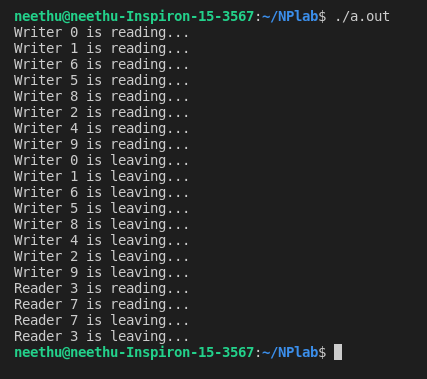
\includegraphics[scale=0.8]{img/e6.png}
\end{figure}
\newpage
\subsection{Result}
Implemented the program for the Second Readers-Writers problem using C language in Ubuntu 20.04 with kernel and the above outputs were obtained.

